\documentclass[../main.tex]{subfiles}

\graphicspath{{../images/}}

\begin{document}
\pagestyle{fancy}
\lhead{Lecture 1: 1/16/24}
\chead{Chapter 1}
\rhead{PHYS 472}
% vertical bar
\section*{Chapter 1: Crystal Structure}
% add to table of contents
\addcontentsline{toc}{section}{Chapter 1: Crystal Structure}


\paragraph{Ideal crystal is constructed by the infinite repetition of identical structural groups of
atoms.} A group is called the basis. Detecting crystal structure started with x-rays due to the
wavelength of the x-ray ($\approx 1$ angstrom) being comparable to the interatomic spacing in a crystal.

\paragraph{What is a \emph{lattice}?}

2D Bravais Lattices \href{https://en.wikipedia.org/wiki/Bravais_lattice}{Wikipedia}
The gamous graphene has a hexagonal (honeycomb structure) like lattice, but it does not have the 
center atom from the true hexagonal lattice. The primitive of this lattice is made of up two atoms
than can be translated to form the lattice. Thus graphene is like a diatomic crystal. 

\paragraph{3D Bravais Lattices} There are 14 Bravais lattices in 3D. In both 2D and 3D, the primitive
cells that make up the lattice must fill the least amount of space and have no `holes' or `extras' left
over. The 2 most common lattices now are the Primitive Hexagonal for its symmetry and the Body
Centered Cubic (BCC) which is the lattice of Silicon, the most important material today. 

\paragraph{Example Structures}
% figure of nacl.png and cscl.png
\begin{figure}[ht]
    \centering
    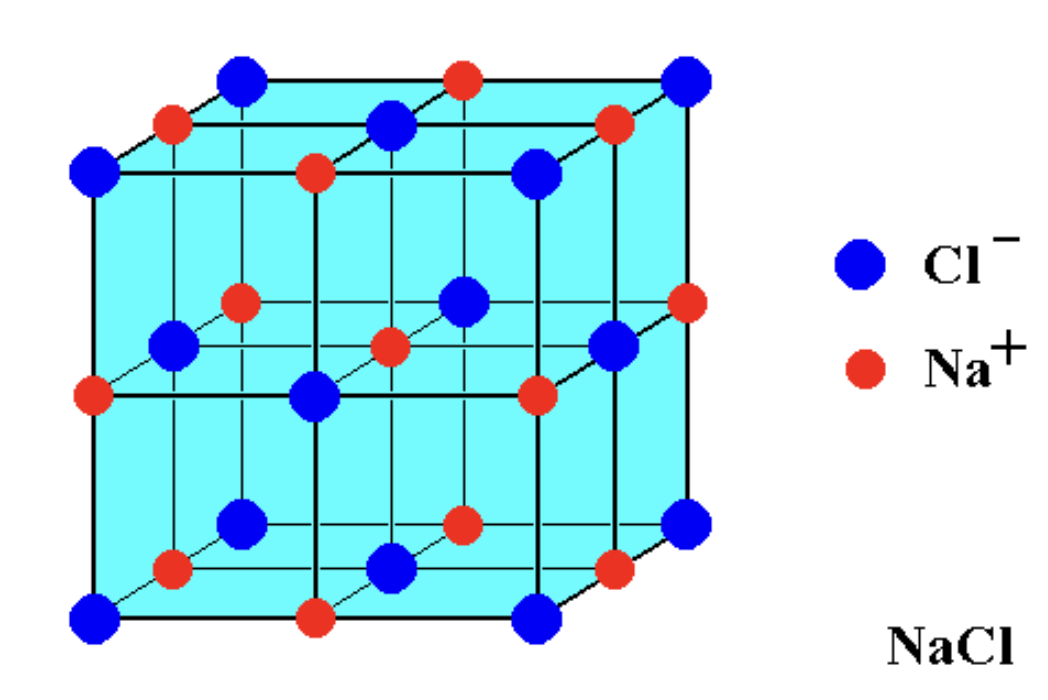
\includegraphics[scale=0.3]{nacl.png}
    \caption{Sodium Chloride Structure (FCC)}
    \label{fig:1.1}
\end{figure}

The lattice of Sodium Chloride is FCC as shown in Figure \ref{fig:1.1}

\begin{figure}[ht]
    \centering
    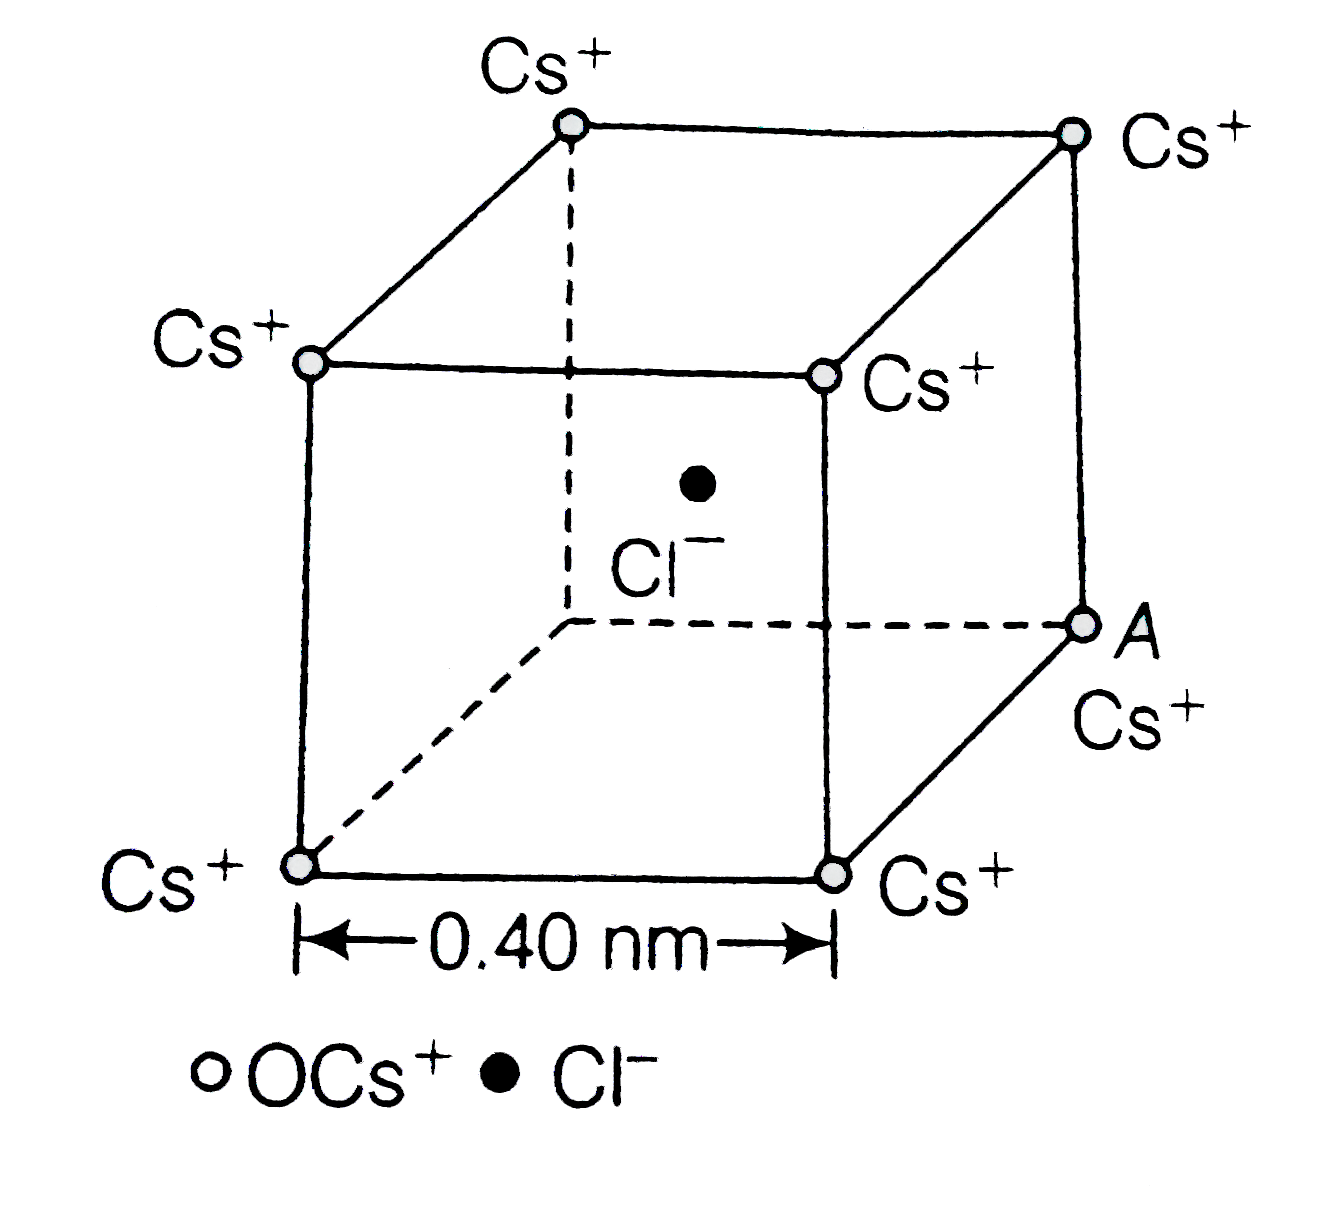
\includegraphics[width=0.3\linewidth]{cecl.png}
    \caption{Cesium Chloride Structure (SC)}
    \label{fig:1.2}
\end{figure}

Figure \ref{fig:1.2} shows the lattice of Cesium Chloride which is SC.

\end{document}